\autoref{fig:mini-full} is a complete representation of the AKF
architecture, excluding labels. The remaining diagrams in this appendix
chapter focus on individual modules in greater detail;
\autoref{fig:mini-full} is intended to help the reader understand the
relationships between individual sub-diagrams, which contain the labels
omitted from this figure.

The following conventions are used for all architectural figures
throughout this thesis, including those below:

\begin{itemize}
\tightlist
\item
  Elements with a \textbf{solid border} refer to AKF submodules, which
  contain processing logic.
\item
  Elements with a \textbf{dotted border} refer to inputs, such as
  scripts and images, that should be used to construct a dataset.
\item
  Elements with a \textbf{dashed border} refer to outputs, such as disk
  images and memory dumps, that should be included with a complete
  dataset.
\end{itemize}

In general, colored boxes refer to a distinct module. The sole exception
is the \emph{translation unit} (colored green), which is distinctly
colored from other submodules due to its complexity.

\begin{figure}[h]
\centering
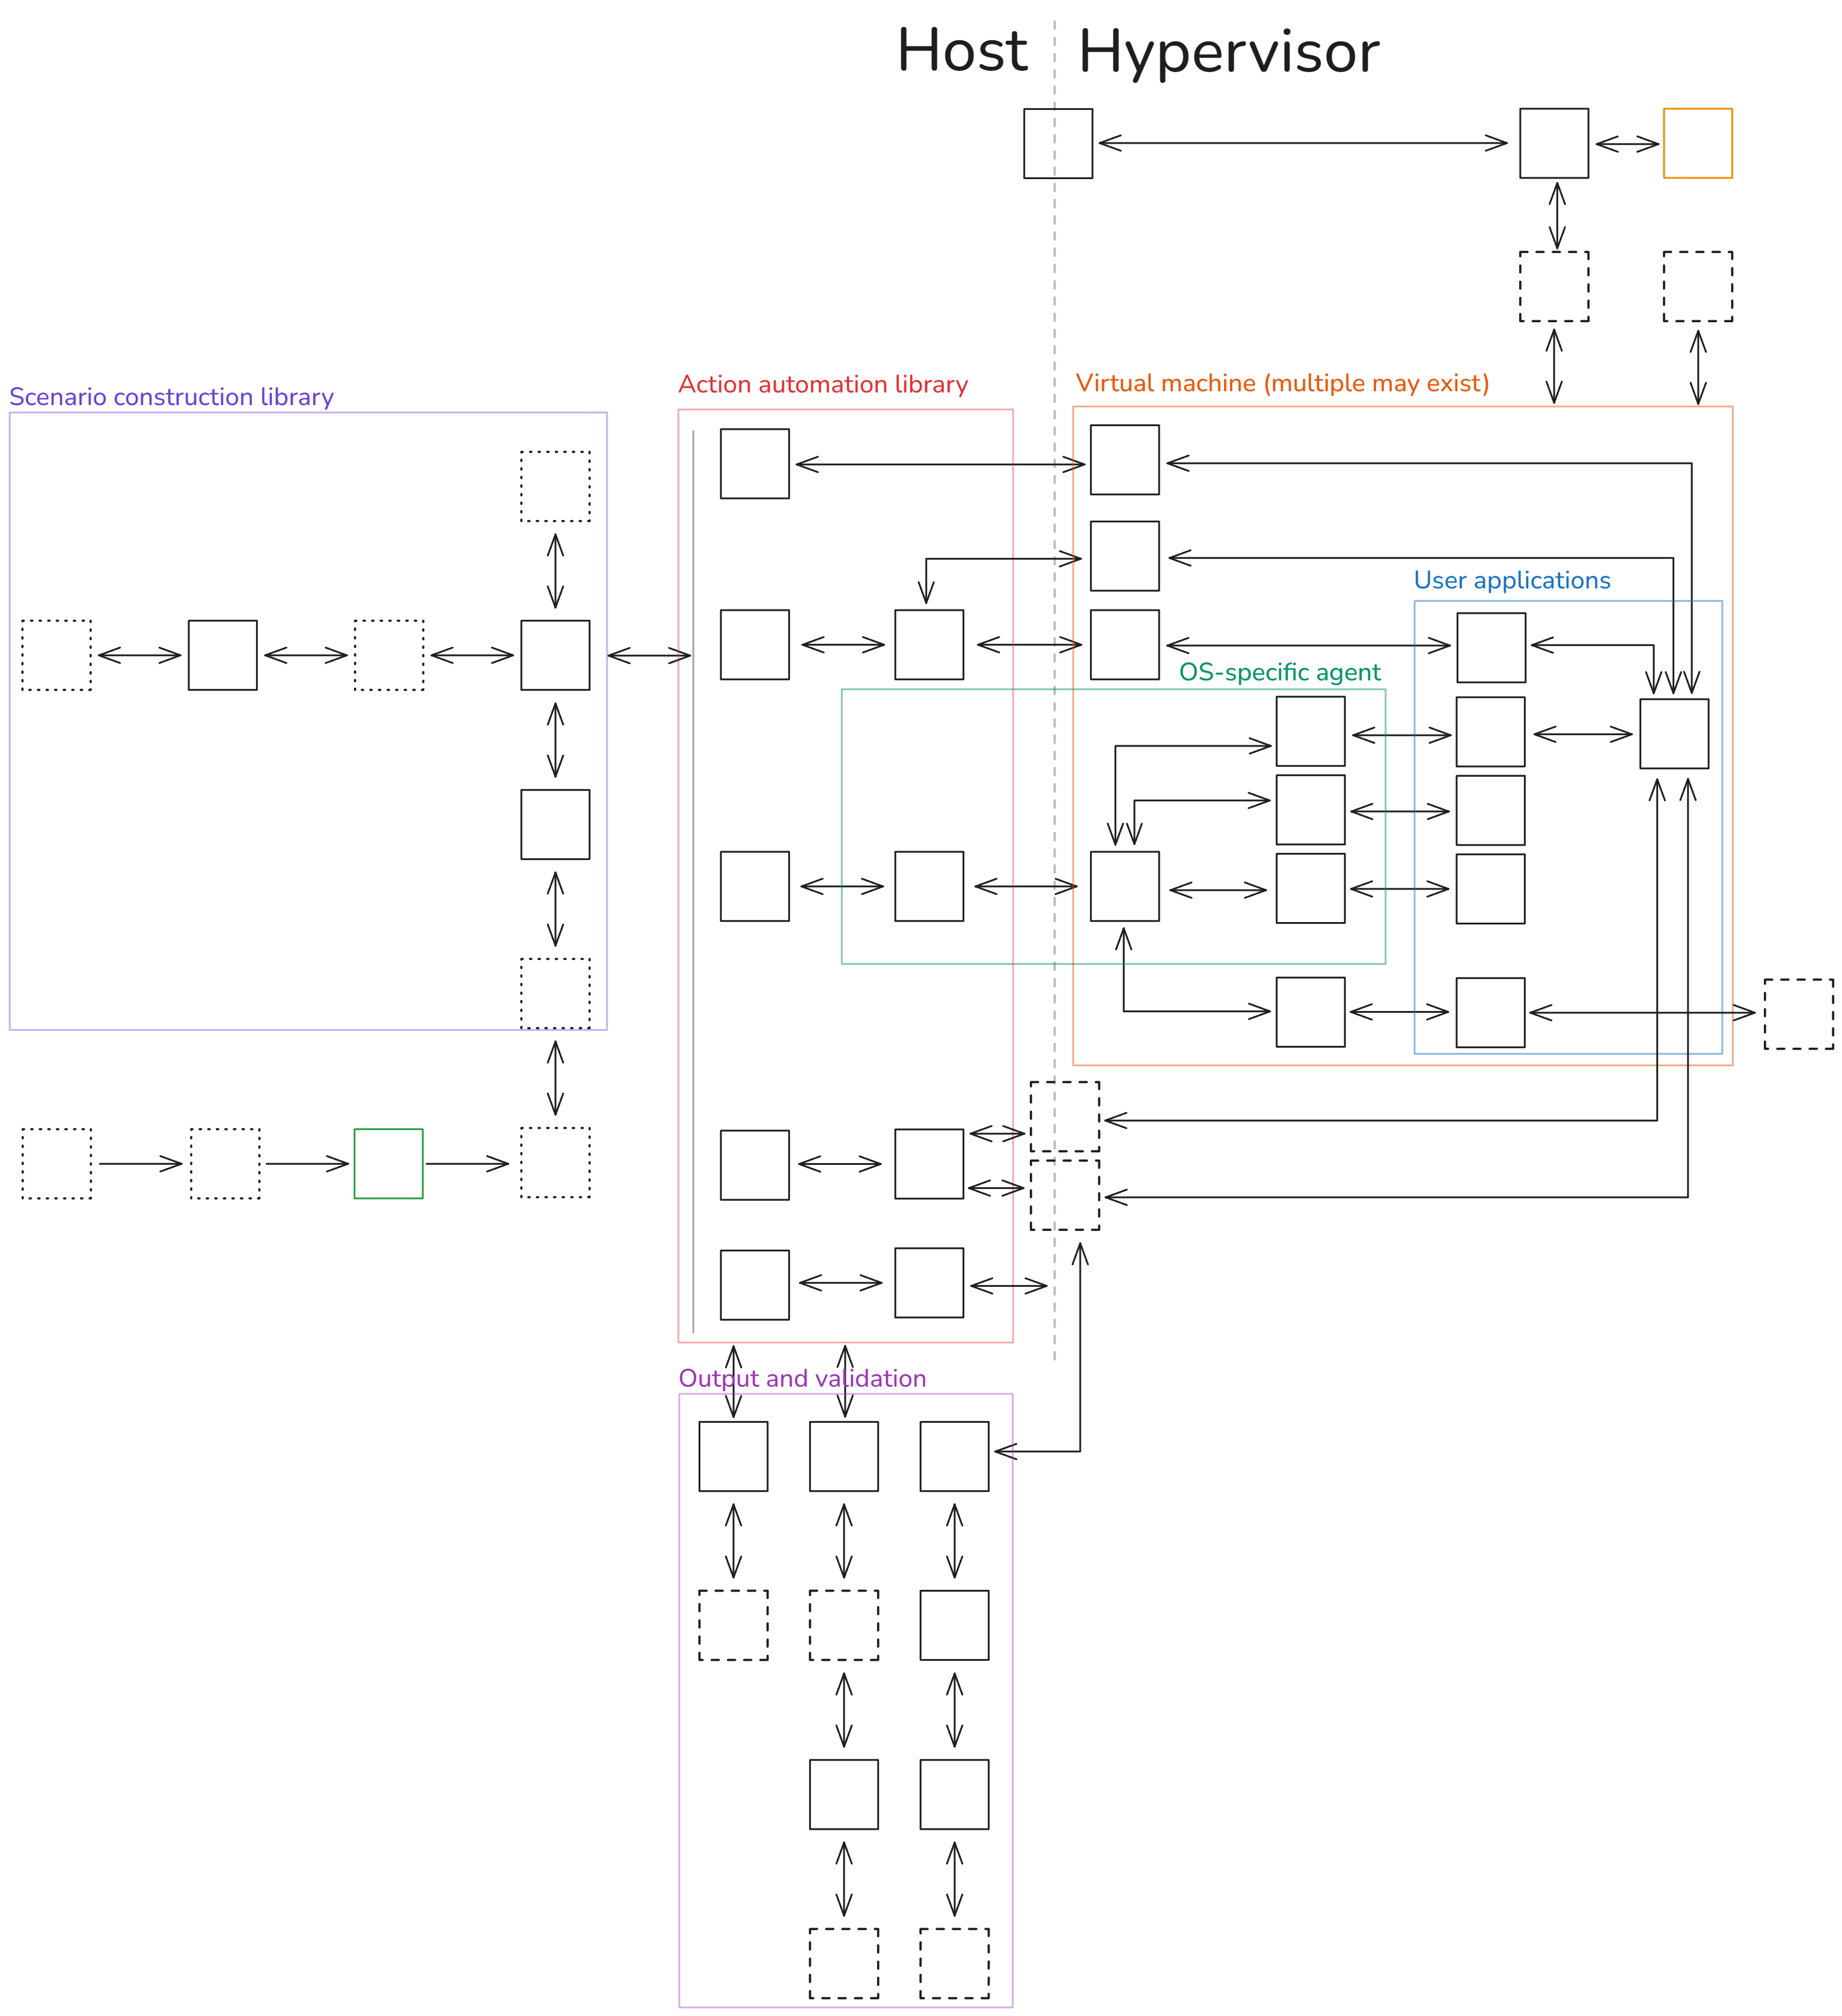
\includegraphics[width=1\linewidth]{mini-architecture-full.png}
\caption{Complete diagram of AKF modules without
labels}\label{fig:mini-full}
\end{figure}

The action automation library, described throughout \autoref{chapter-four}, is depicted in \autoref{fig:architecture-full-b}.

\begin{figure}[h]
\centering
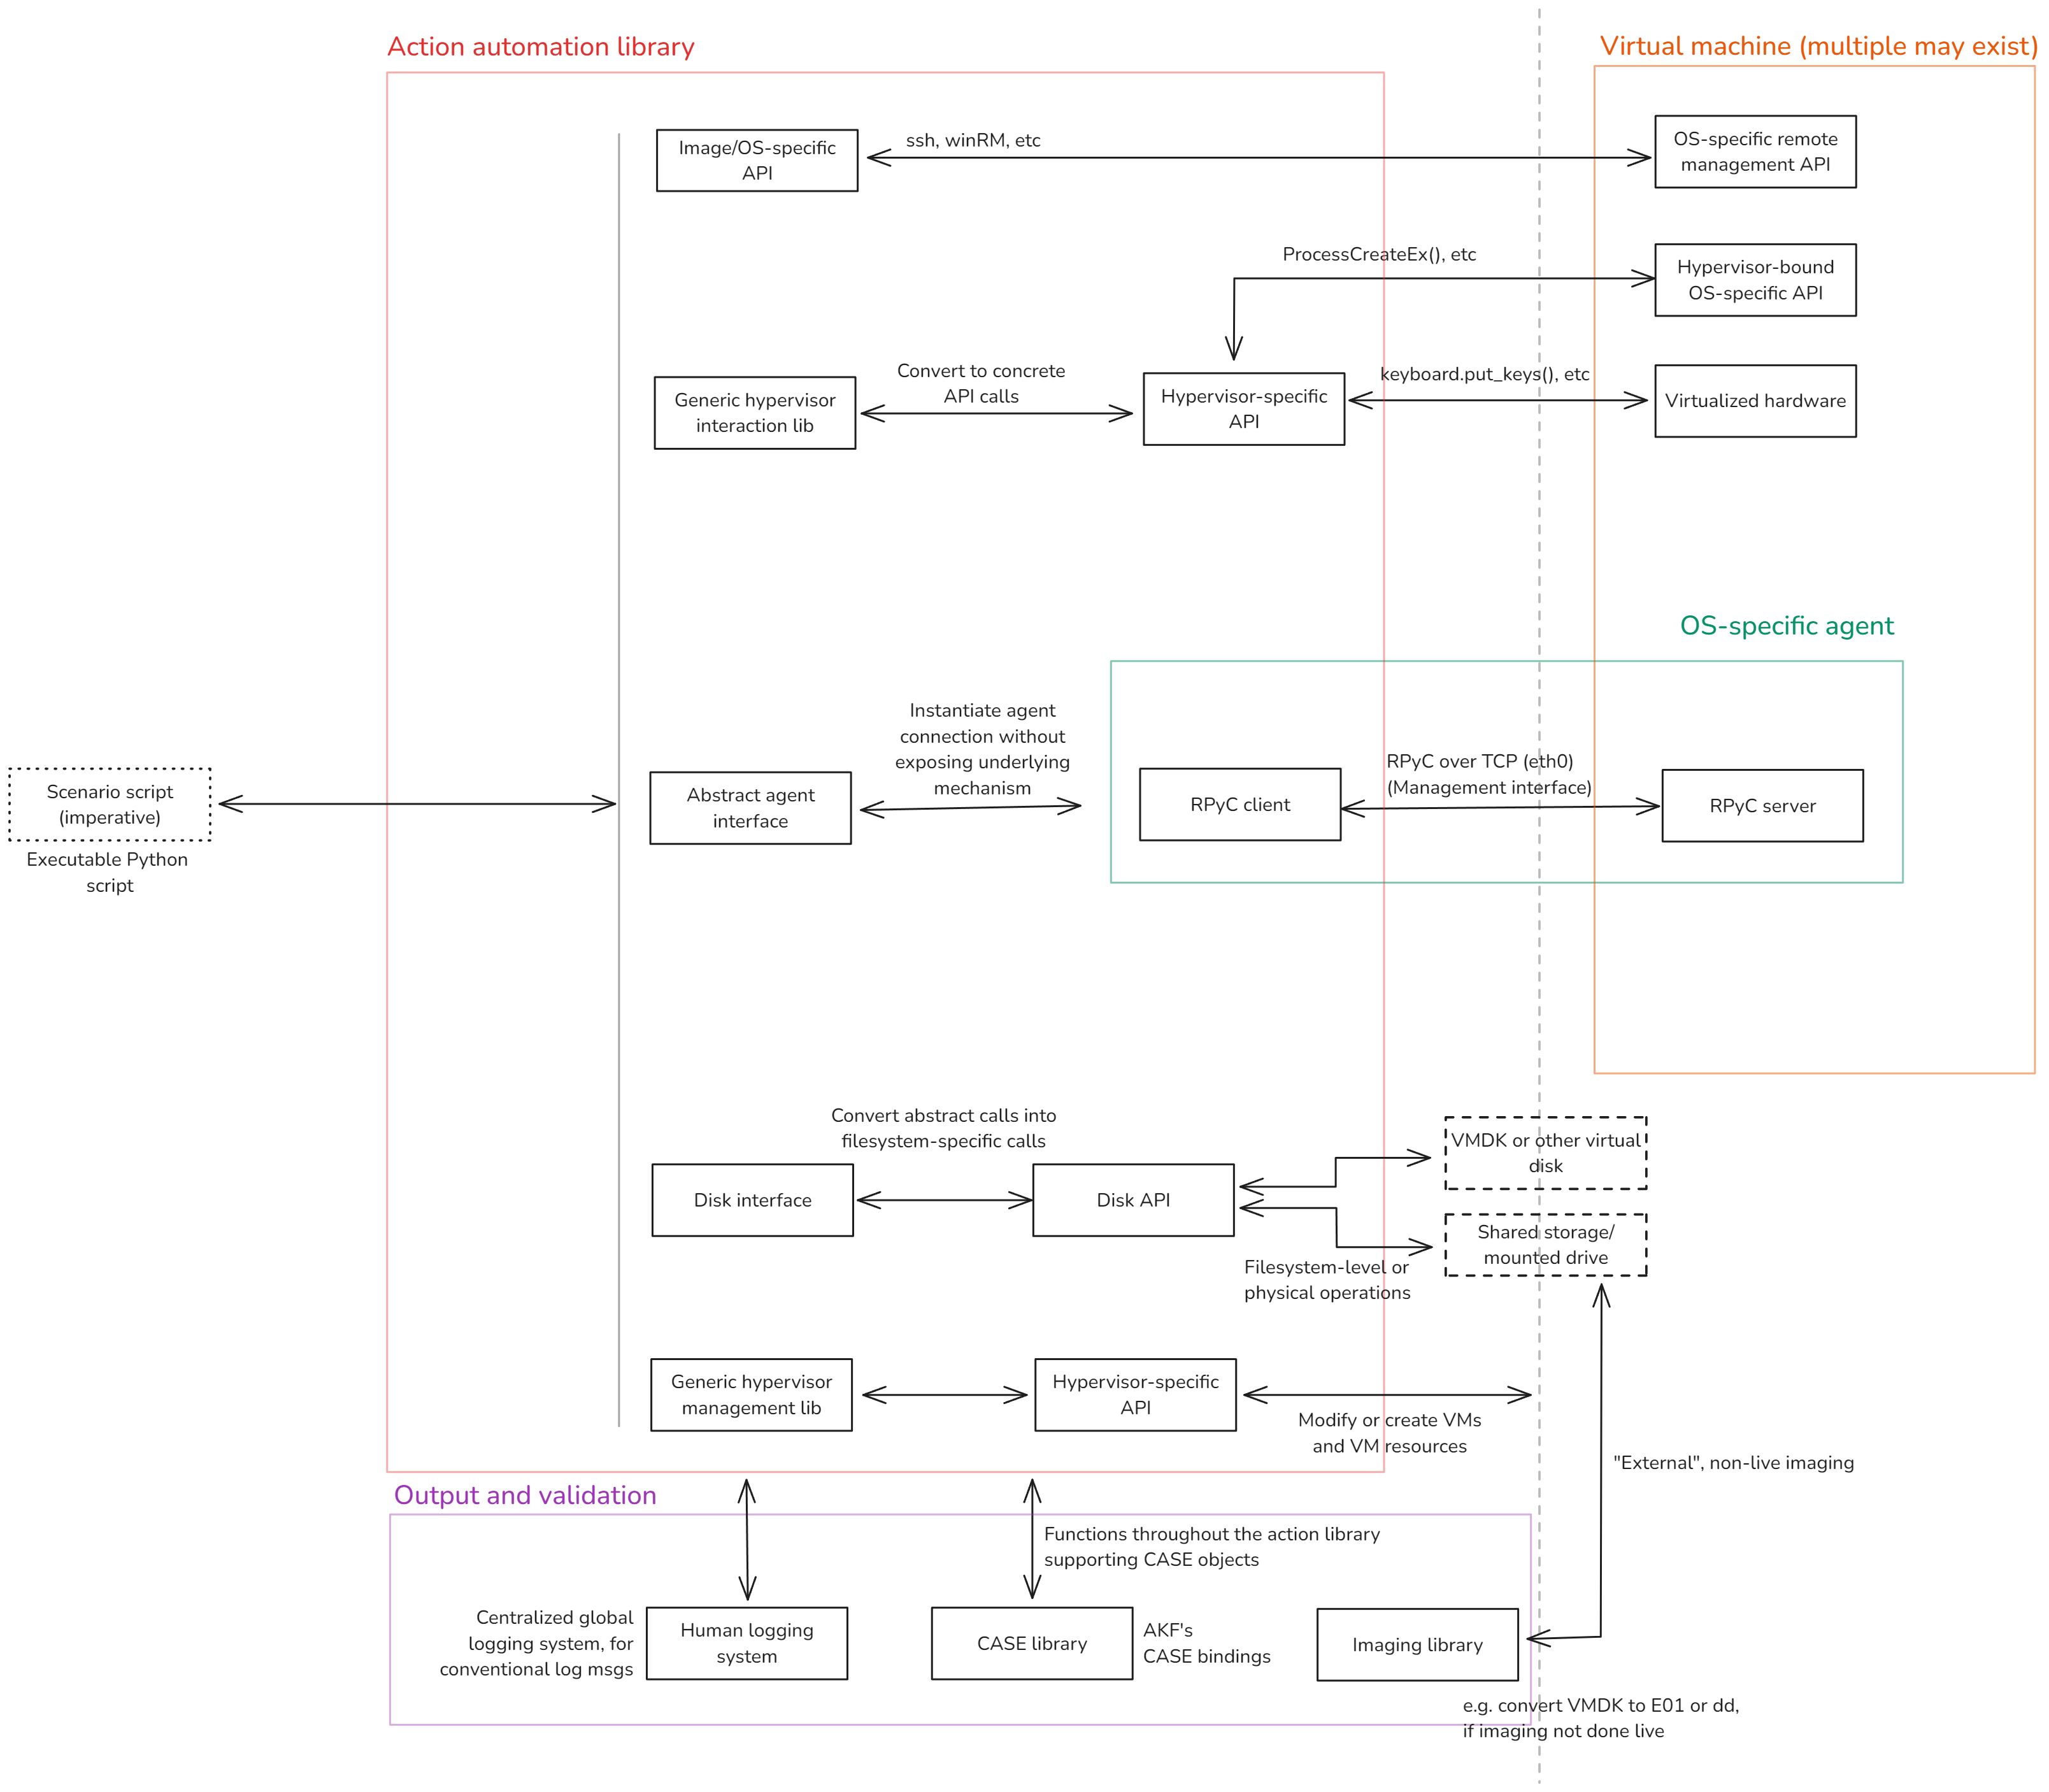
\includegraphics[width=1\linewidth]{architecture-full-b.png}
\caption{Detailed diagram of \passthrough{\lstinline!akflib!} and
related modules}\label{fig:architecture-full-b}
\end{figure}

The virtualized environment and its agent, also described throughout
\autoref{chapter-four}, is depicted in
\autoref{fig:architecture-full-d}. Note that some elements depicted in
this figure are described in \autoref{chapter-five} and
\autoref{chapter-six}.

\begin{figure}[h]
\centering
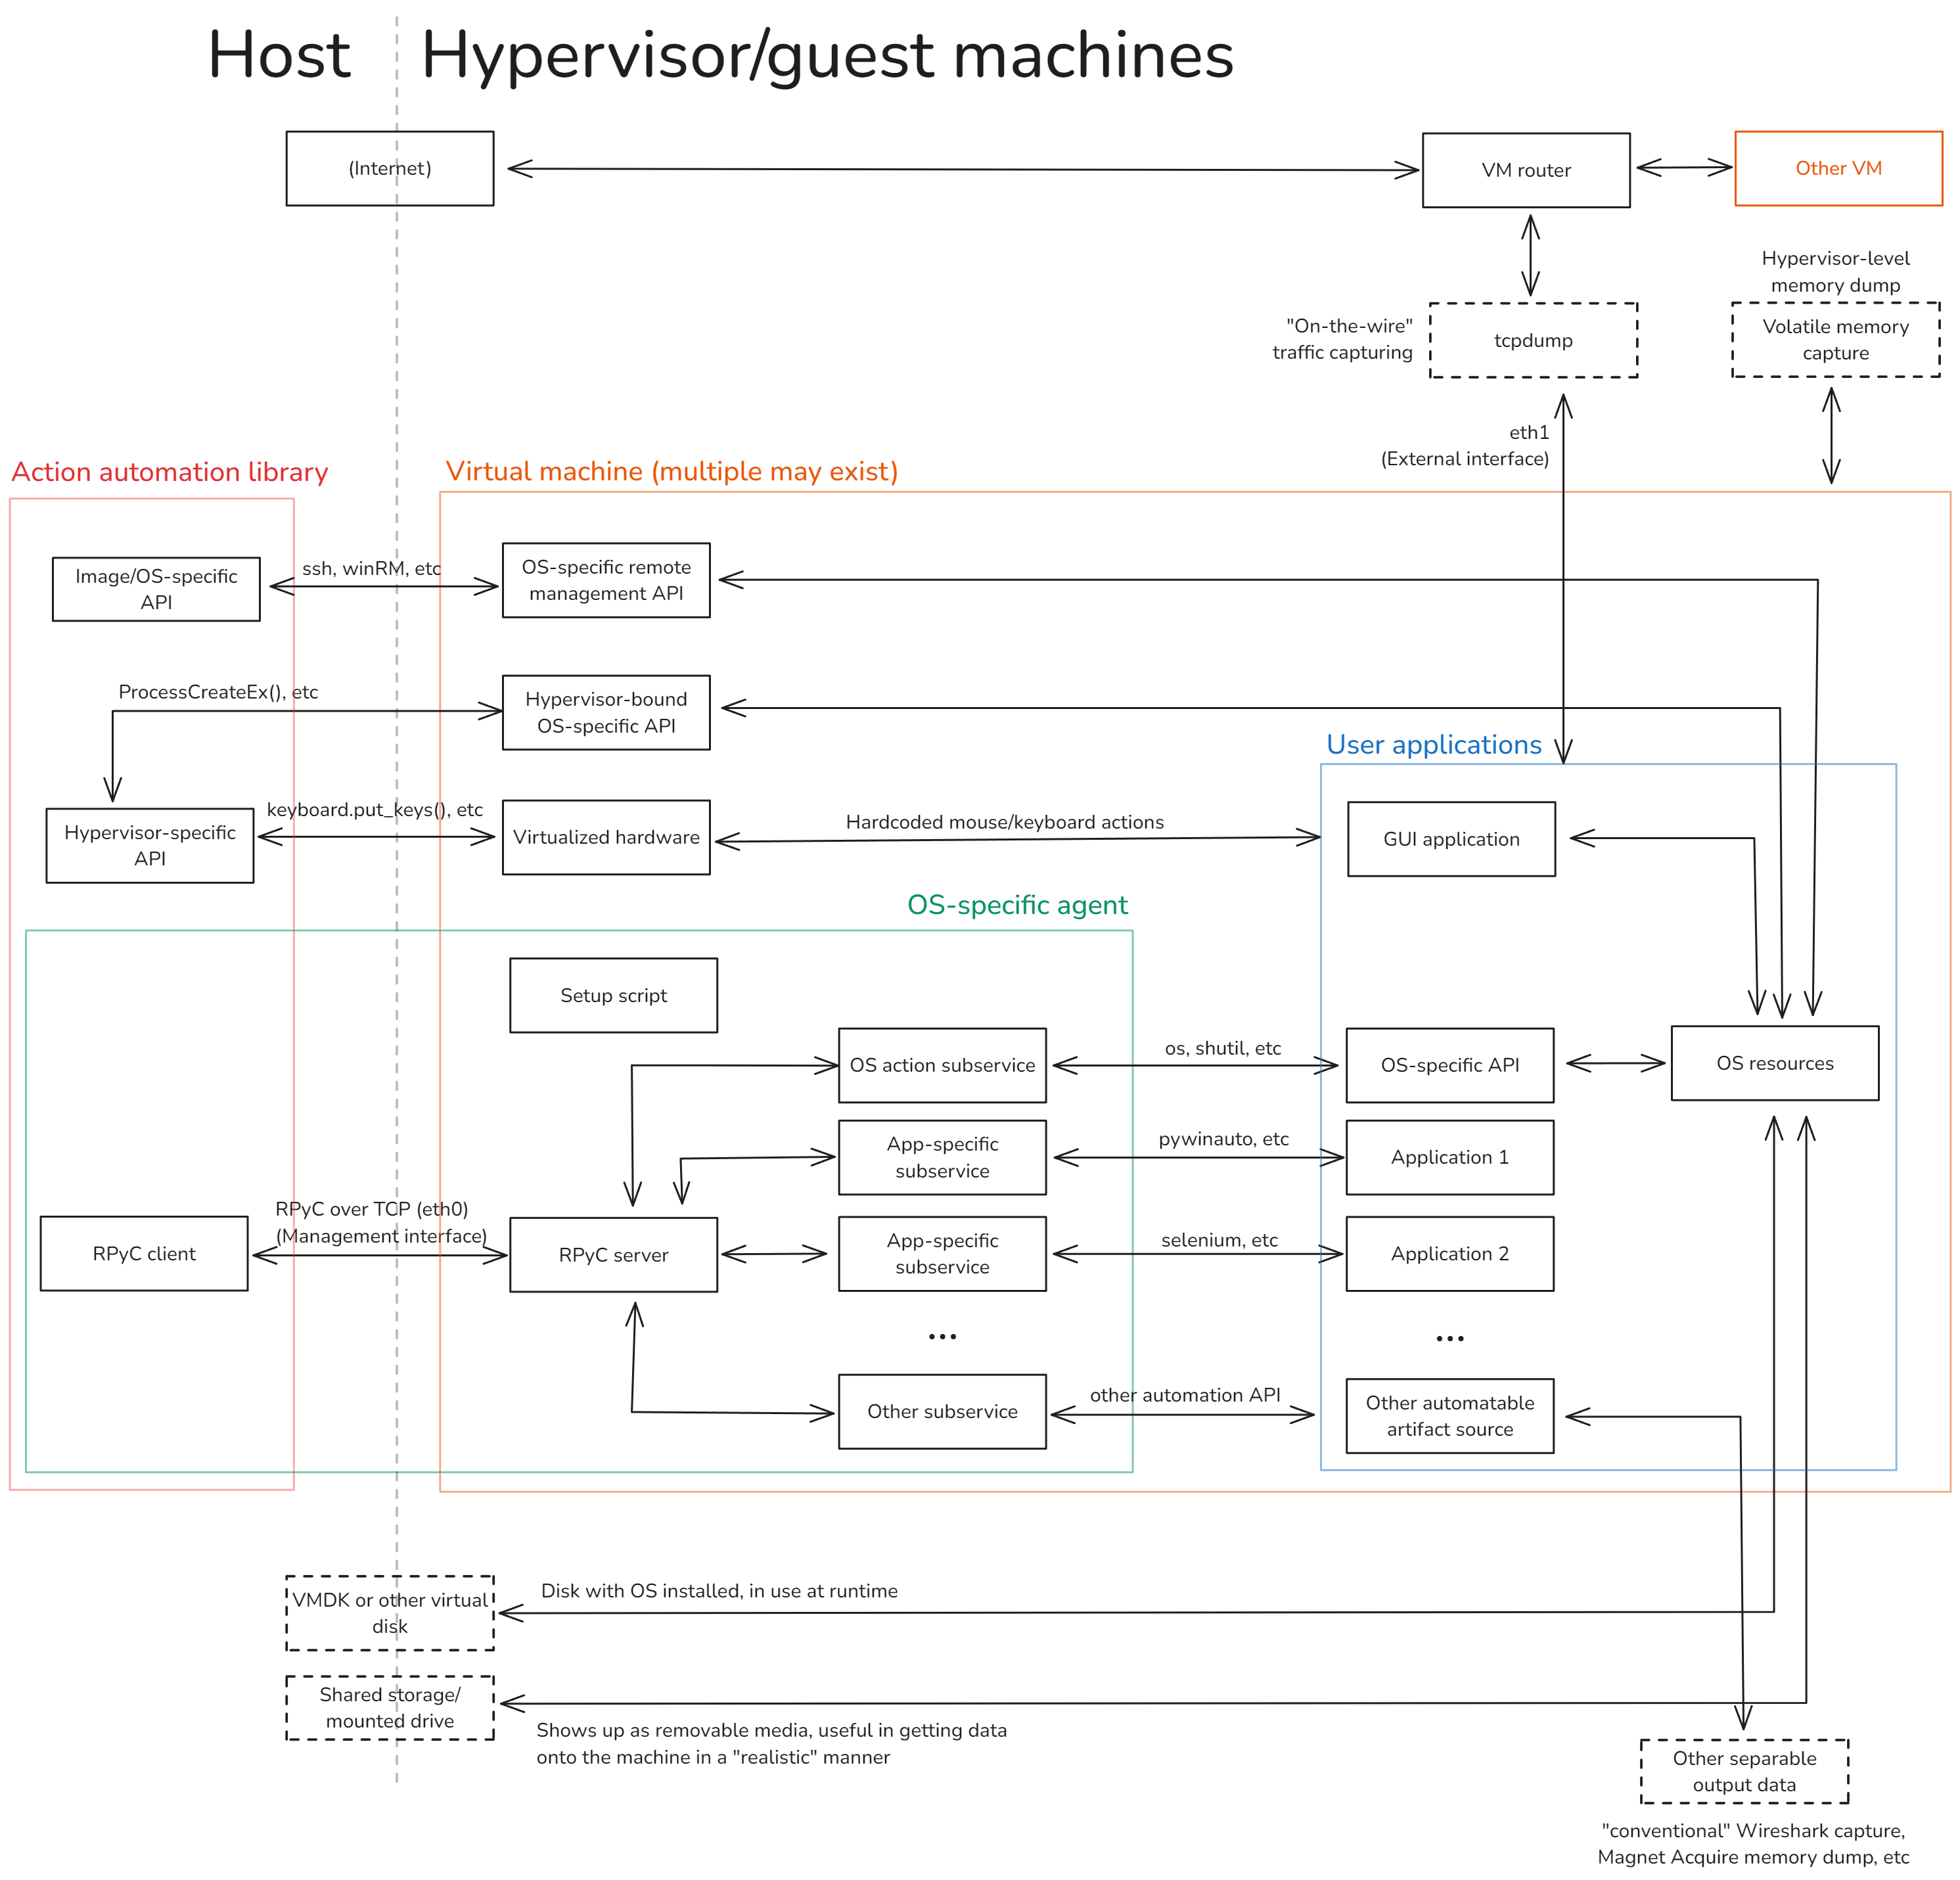
\includegraphics[width=1\linewidth]{architecture-full-d.png}
\caption{Detailed diagram of AKF's virtualized
environment}\label{fig:architecture-full-d}
\end{figure}

The output and validation library, described throughout \autoref{chapter-five}, is depicted in
\autoref{fig:architecture-full-c}. Note that this is distinct from
\autoref{fig:output-full}, which includes various virtual machine
outputs due to their role in the chapter's discussion.

\begin{figure}[h]
\centering
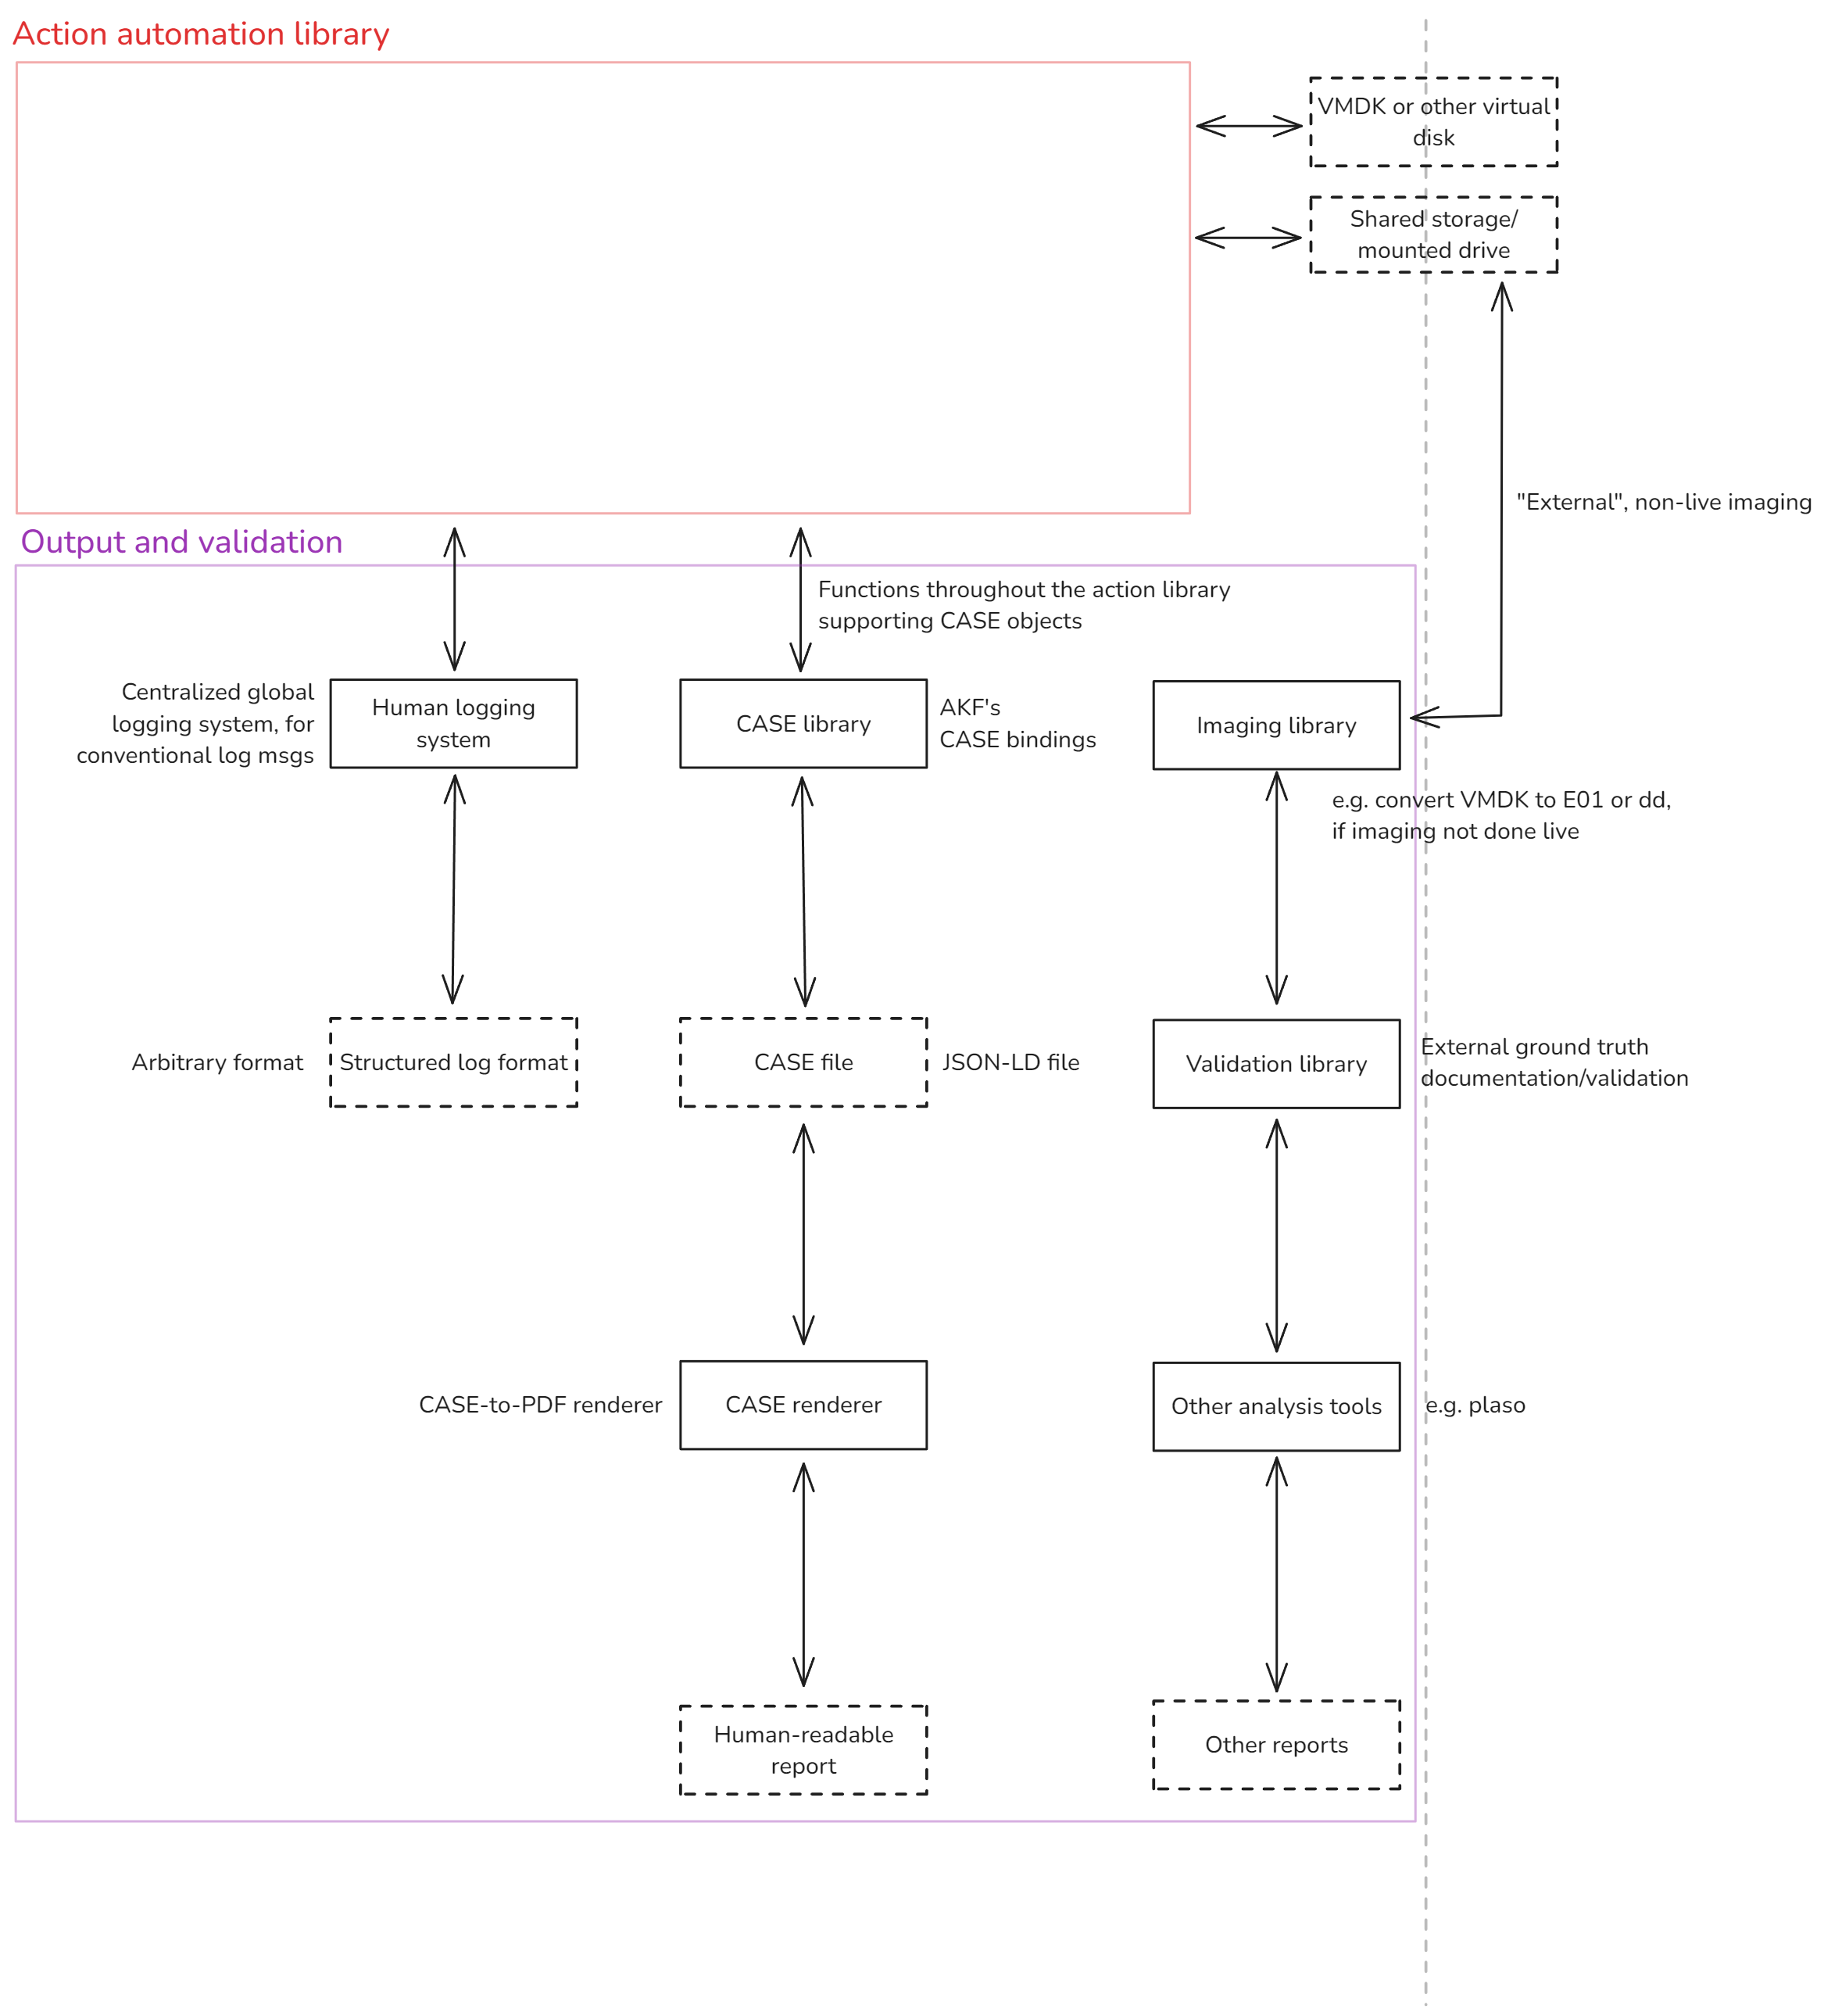
\includegraphics[width=1\linewidth]{architecture-full-c.png}
\caption{Detailed diagram of AKF modules responsible for output and
validation}\label{fig:architecture-full-c}
\end{figure}

Finally, modules related to scenario construction, as described in
\autoref{chapter-six}, are depicted in
\autoref{fig:architecture-full-a}.

\begin{figure}[h]
\centering
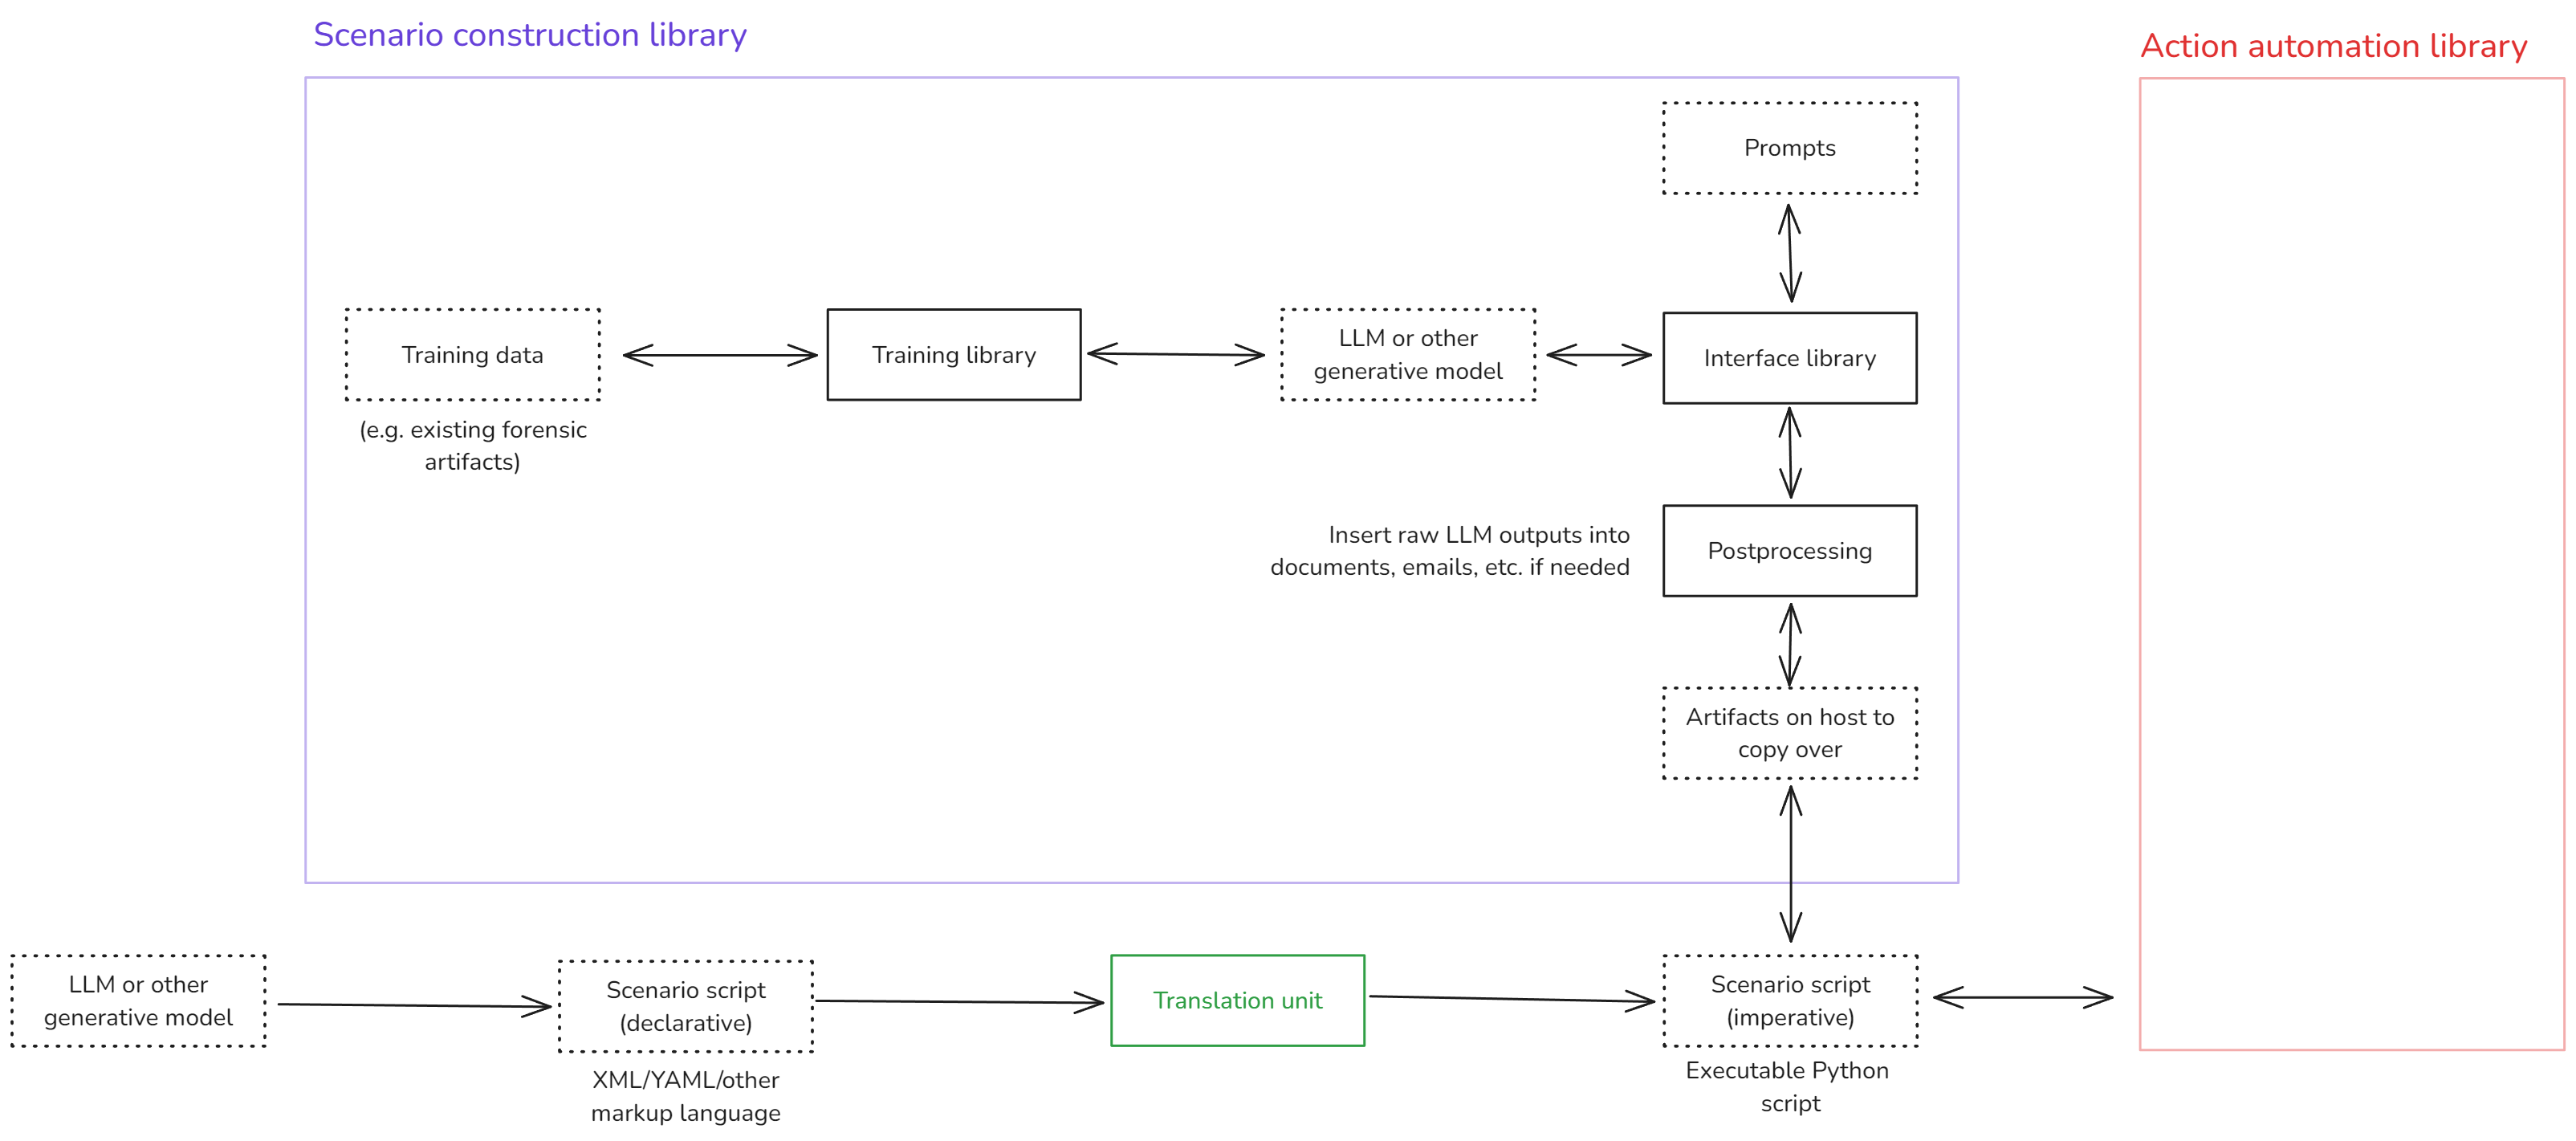
\includegraphics[width=1\linewidth]{architecture-full-a.png}
\caption{Detailed diagram of AKF modules related to scenario
construction}\label{fig:architecture-full-a}
\end{figure}
